\documentclass[a4paper]{article}

\usepackage[french]{babel}
\usepackage[utf8]{inputenc}
\usepackage[T1]{fontenc}
\usepackage{fullpage}
\usepackage{hyperref}
\usepackage{graphicx}

\author{Titouan \bsc{Christophe}}
\title{Synthèse de bases de données}
\date{\today}

\begin{document}
\maketitle
\tableofcontents

\section{Modèle entité-relation}
Un schéma conceptuel des données, pas forcément implémenté de cette façon.

\subsection{Entité}
\begin{figure}[h!]
    \center
    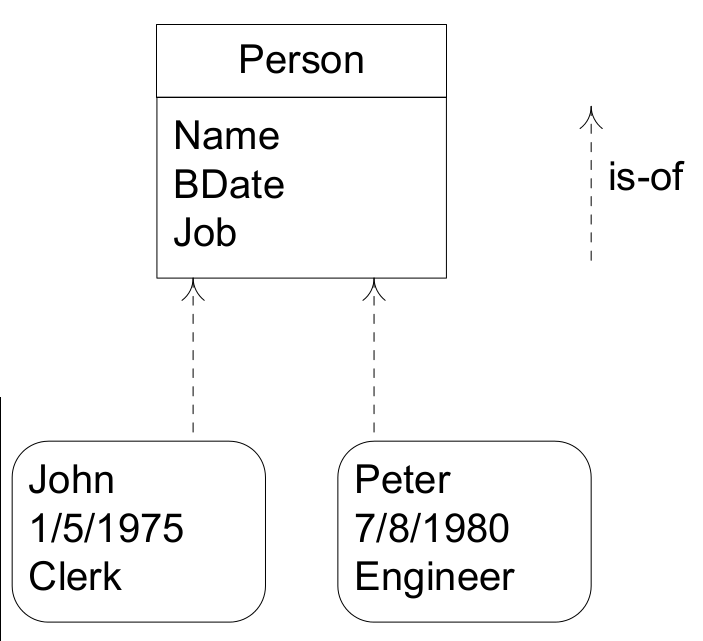
\includegraphics[width=.3\textwidth]{fig/entity.png}
    \caption{Une entité}
\end{figure}

Selon le contexte, désigne la classe (modèle) ou l'objet (l'instance).

\subsection{Relation}
\begin{figure}[h!]
    \center
    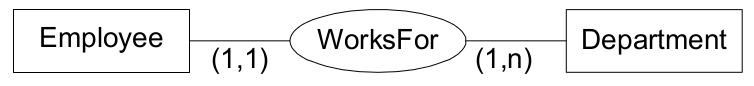
\includegraphics[width=.7\textwidth]{fig/relation.png}
    \caption{\label{fig:relation}Une relation One-to-many}
\end{figure}
\begin{itemize}
  \item On doit spécifier l'arité minimale et maximale pour chaque pair de la relation
  \item La relation porte un nom (souvent dans un seul sens)
  \item \textbf{One-to-one}, \textbf{one-to-many} ou \textbf{many-to-many}
\end{itemize}
\subsubsection{Vision ensembliste}
\begin{figure}[h!]
    \center
    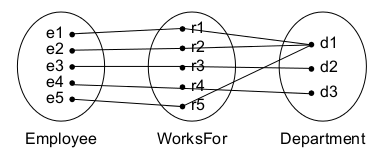
\includegraphics[width=.3\textwidth]{fig/relation-ensembliste.png}
    \caption{Vue ensembliste de la relation à la Figure \ref{fig:relation}}
\end{figure}

\end{document}